\documentclass[12pt,a4paper]{report}
\usepackage[utf8]{inputenc}
\usepackage[T1]{fontenc}
\usepackage{fontspec}
\usepackage[polish]{babel}
\usepackage{amsmath}
\usepackage{graphicx}
\usepackage[table,xcdraw]{xcolor}
\usepackage{hhline}
\usepackage{placeins}
\usepackage[margin=0.6in]{geometry}
\usepackage{appendix}
\usepackage{colortbl}
\usepackage{physics}
\usepackage{float}
\usepackage{datetime}
\usepackage{makeidx}

% folowing  must be in this order
% \usepackage{varioref}
\usepackage{hyperref}
% \usepackage{cleveref}

\title{Termodynamika R 2021/2022}
\author{Kacper Cybiński}
% \newdate{date}{28}{01}{2022}
% \date{\displaydate{date}}
\date{\today}
\makeindex
\setlength\parindent{0pt}

\addto\captionspolish{\renewcommand{\chaptername}{Lecture}}

\newcommand{\ind}[1]{{\color{blue} #1\index{#1}}}

\newcommand{\com}[1]{{\color{red} #1}}

\newcommand{\link}[2]{{\color{cyan} \href{#1}{#2}}}

\renewcommand{\emph}{\textbf}

\newenvironment{lecture}[1][]{\par\medskip
   \noindent\chapter \rmfamily}{\medskip}

\begin{document}

\maketitle

% ---------------------------------------------------------------------------
% Wykład 01.03.2022

\chapter*{Organizacja wykładu}:
\begin{enumerate}
    \item Dwa kolokwia - po 40 \% pkt
    \item Zadania domowe - 20 \% pkt
\end{enumerate}

{\color{blue} \link{http://www.fuw.edu.pl/~piotrek/stat2022}{Strona wykładu}}

Suma - 100 \%. Zaliczenie ćwiczeń $> 50 \%$, Egzamin 100 \%. Propozycja oceny w zakresie $3-4.5$ Po 5 przychodzimy na ustny. Ustny też dla plebsu, nie tylko dla tych z 4.5 ({\it Patrz Pawełczyk})

Egzamin i kolokwia mają 2 częsci:
\begin{itemize}
\item Test ABCD, 1 lub wielokrotnego wyboru $\sim 45$ min.
\item Zadania - $\sim 3h$
\end{itemize}

Zadania domowe: Jak na elektro, ale tylko 3 zadania na tydzień. Na wykładzie czwartkowym losowanie zadania zbieranego. Jest jedno dodatkowe, trudniejsze, "Joker".

\begin{lecture}
\section{\ind{Problem wielu ciał}}

Dla problemu 3 ciał pierwsze znalezione stabilne rozwiązanie zostało opisane przez Lagrange'a. Jest to ruch po okręgu, a w $\sim 1990$ opisano też stabilną orbitę po ósemce.

Historia superkomputerów:
\begin{itemize}
    \item Anton (2008) - Daniel Shaw
    \begin{itemize}
        \item Problem zwijania białek
        \item 10 ms zwijania - 5 min obliczeń
        \item $10^4-10^5$ atomów - 1 ms w 100 dni. Tj. $10$ ns/dzień
    \end{itemize}
    \item Summit (2018)
    \begin{itemize}
        \item 27 tys. GPU + 9 tys. CPU.
        \item $200\cdot10^6$ 32 ns/dzień
    \end{itemize}
\end{itemize}
Dla skali -> kubek z herbatą ma \textbf{$\sim10^{25}$ atomów}

\ind{Demon Laplace'a}:
Laplace mówił, że symulacja, która by znała położenia i pędy wszyskich cząstek by znała przeszłość i przyszłość $\to$ \textit{przeszłość i przyszłość by stała przed nią otworem}. Jest to wizja świata skrajnie deterministycznego. Obecnie raczej upadłej. {\color{green} Wniosek:} Kupując kefir nie obchodzi nas położenie wszystkich atomów, a właściwości makroskopowe.

\ind{Fizyka statystyczna}: Jest dziedziną zajmującą się przejściem z informacji mikroskopowej do informacji makroskopowej, która jest obiektem naszego zainteresowania.

\begin{figure}[!ht]
    \centering
    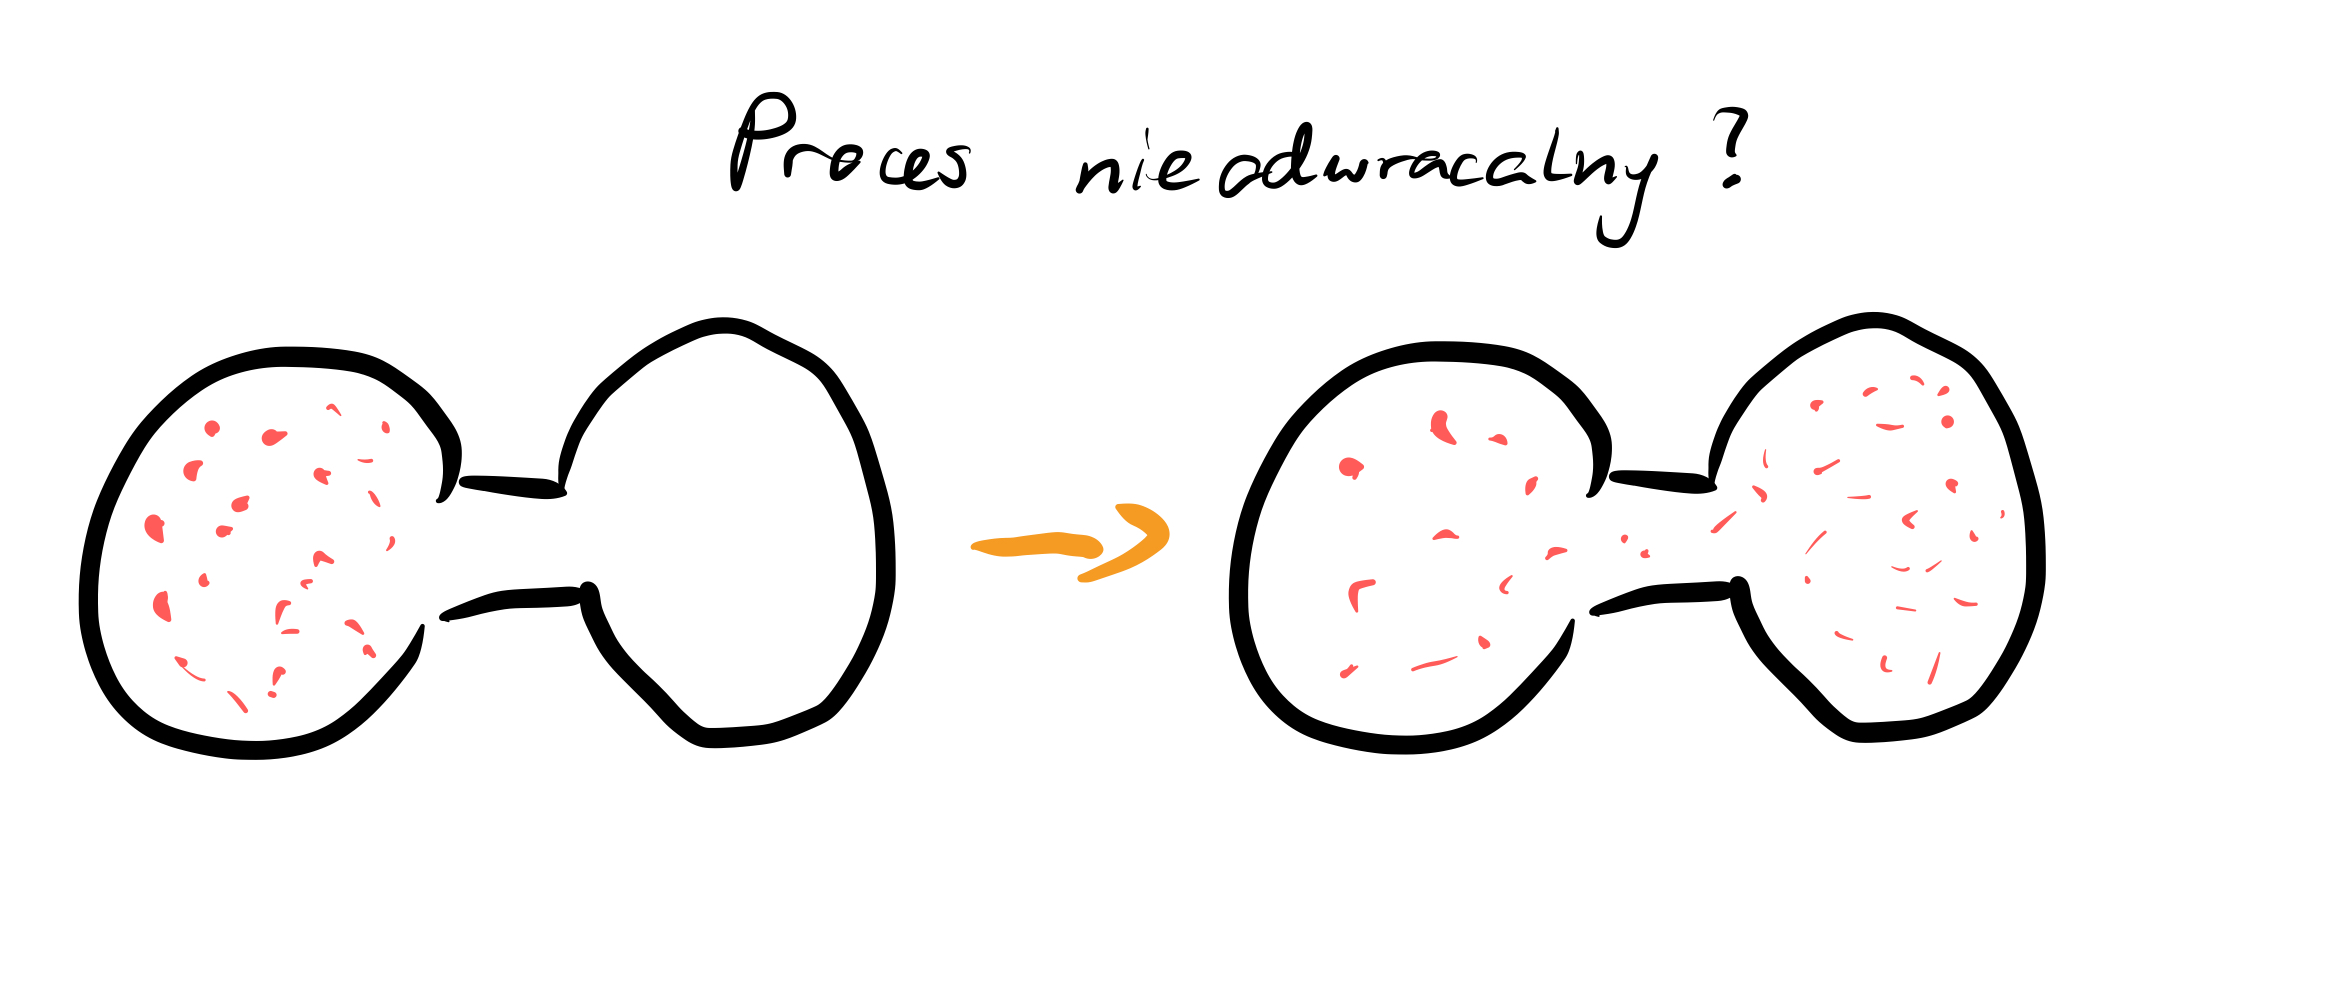
\includegraphics[width=0.8\linewidth]{Wyk_1_Rys_1.jpeg}
    \caption{Proces nieodwracalny?}
\end{figure}

\FloatBarrier

\section{Pokazy}
\subsection{Cylindry z ulepkiem cukru}
Widzimy tu na demonstracji \ind{odwracalność}. Są dwa rodzaje:
\begin{itemize}
    \item {\color{blue} odwracalność dynamiczna} \index{odwracalność!dynamiczna}:
    \[m \dv{v}{t} = F\]
    Wynika ona z dynamiki Newtonowskiej, jest symetryczna względem transformacji $t \to -t$, $v \to -v$.
    \item {\color{blue} odwracalność kinematyczna} \index{odwracalność!kinematyczna}:
    \[0 = m \dv{v}{t} = F - \gamma v \implies v = \frac{F}{\gamma}\]
    Gdzie $\gamma$ jest współczynnikiem oporu. Ta odwracalnośc jest symetryczna względem przekształcenia $F \to -F, v \to -v$. Ten rodzaj odwracalności zachodzi w lepkich cieczach. Symetryczny względem zmiany kierunku siły i prędkości, ale z czasem nieodwracalnym.
\end{itemize}

\begin{figure}[!ht]
    \centering
    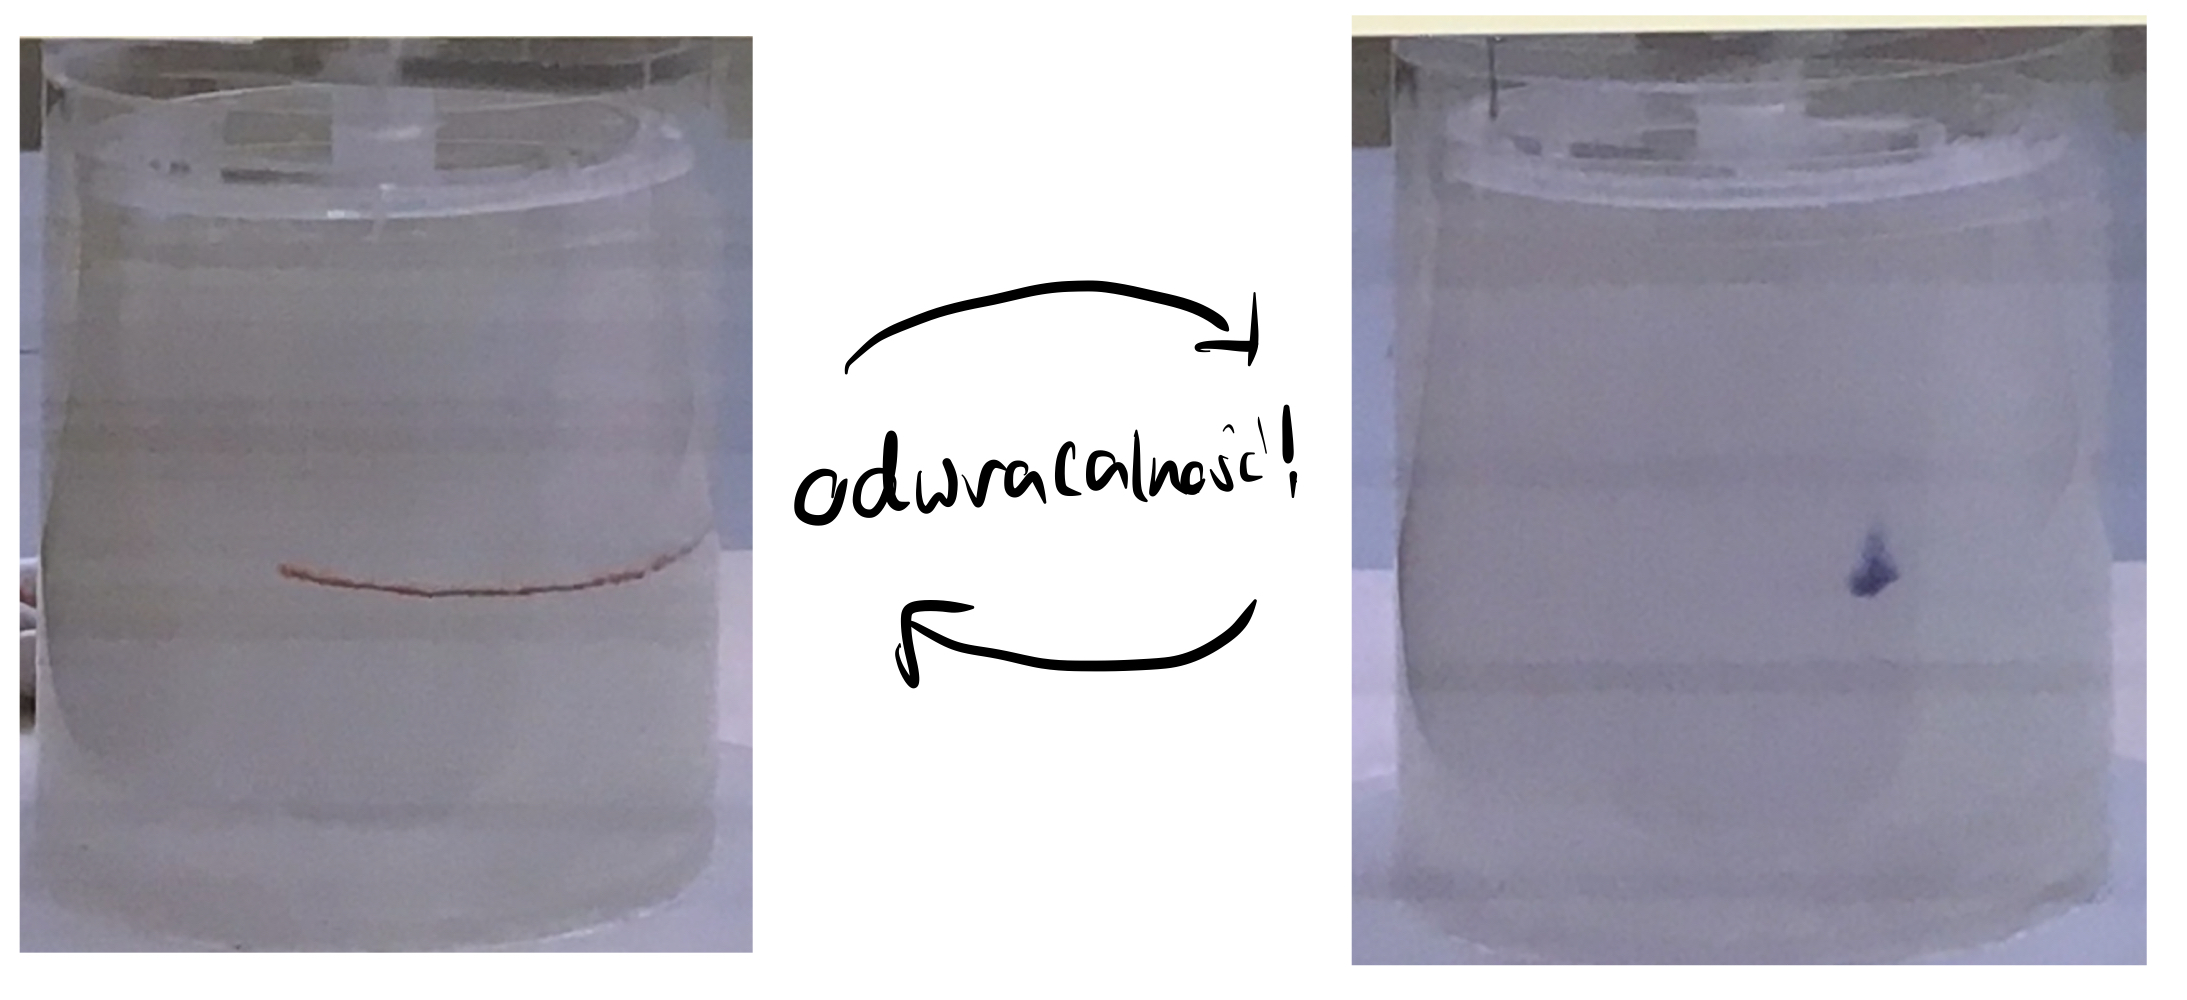
\includegraphics[width=0.8\linewidth]{Wyk_1_Rys_2.jpeg}
    \caption{Demonstracja odwracalności kinematycznej. Działa to tylko dla \emph{lepkiej cieczy}}
    \label{fig:lec_1:odwracalność}
\end{figure}

\begin{figure}[!ht]
    \centering
    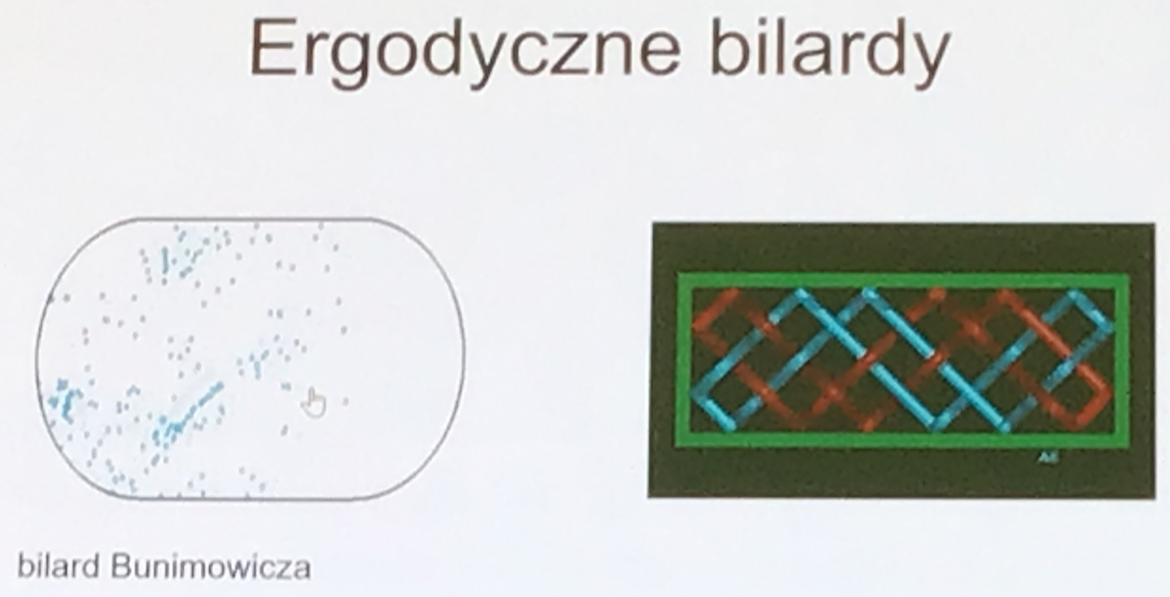
\includegraphics[width=0.8\linewidth]{Wyk_1_Rys_3.jpeg}
    \caption{Demonstracja \emph{Bilardu Bunimowicza}. Po prawej bilard prostokątny - Nie Ergodyczny, ponieważ po odpowiednio długim czasie nie uśrednia się rozkład cząstek - Nie osiąga równowagi.}
    \label{fig:lec1:bilardbunimowicza}
\end{figure}

Kolejnym pojęciem które się pojawia jest \ind{ergodyczność}. Oznacza to, że średnia $\expval{x}$ z układu  po czasie jest równa średniej po powierzchni. Przykładem takiego układu jest zasadniczo \emph{Bilard bunimowicza} (Patrz Rysunek \ref{fig:lec1:bilardbunimowicza}). Układ ergodyczny to taki, który po odpowiednio dużym czasie osiąga stan równowagi.


\section{Model Ehrenfestów}
\begin{figure}[!ht]
    \centering
    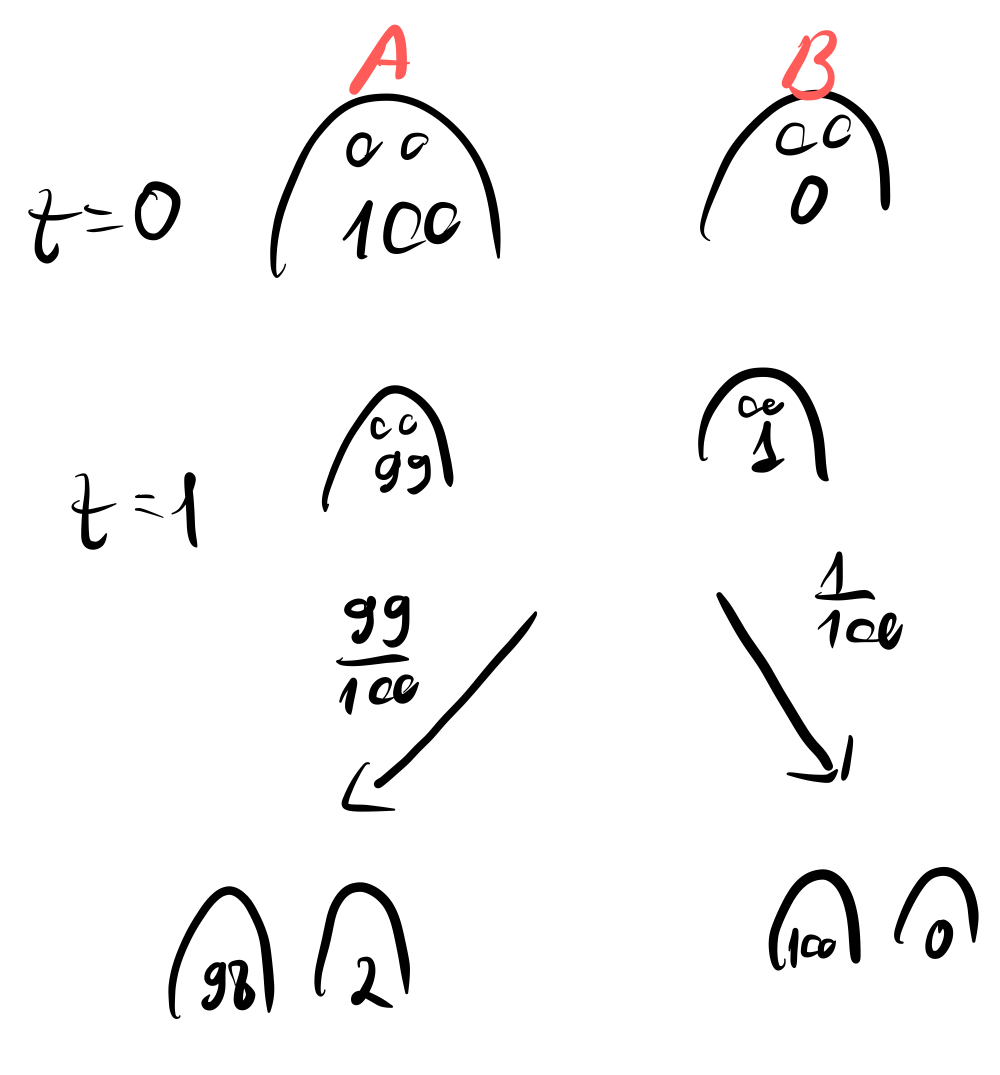
\includegraphics[width=0.8\linewidth]{Wyk_1_Rys_4.jpeg}
    \caption{Demonstracja \emph{Modelu Ehrenfestów}. Bierzemy dwa psy i liczymy sobie $\expval{n_a(t)}$. W tym celu patrzymy sobie na \ind{ansambl} (zespół) dwójek psów.}
    \label{fig:lec_1:pchły}
\end{figure}

\end{lecture}

% --------------------------------------------------------------------------
% Wykład 03.03.2022

\FloatBarrier

\begin{lecture}
\section{Ruch cząstek - Ruchy Browna}

Wprowadzamy sobie jak propaguje się cząstka w cieczy w czasie.

\begin{figure}[!ht]
    \centering
    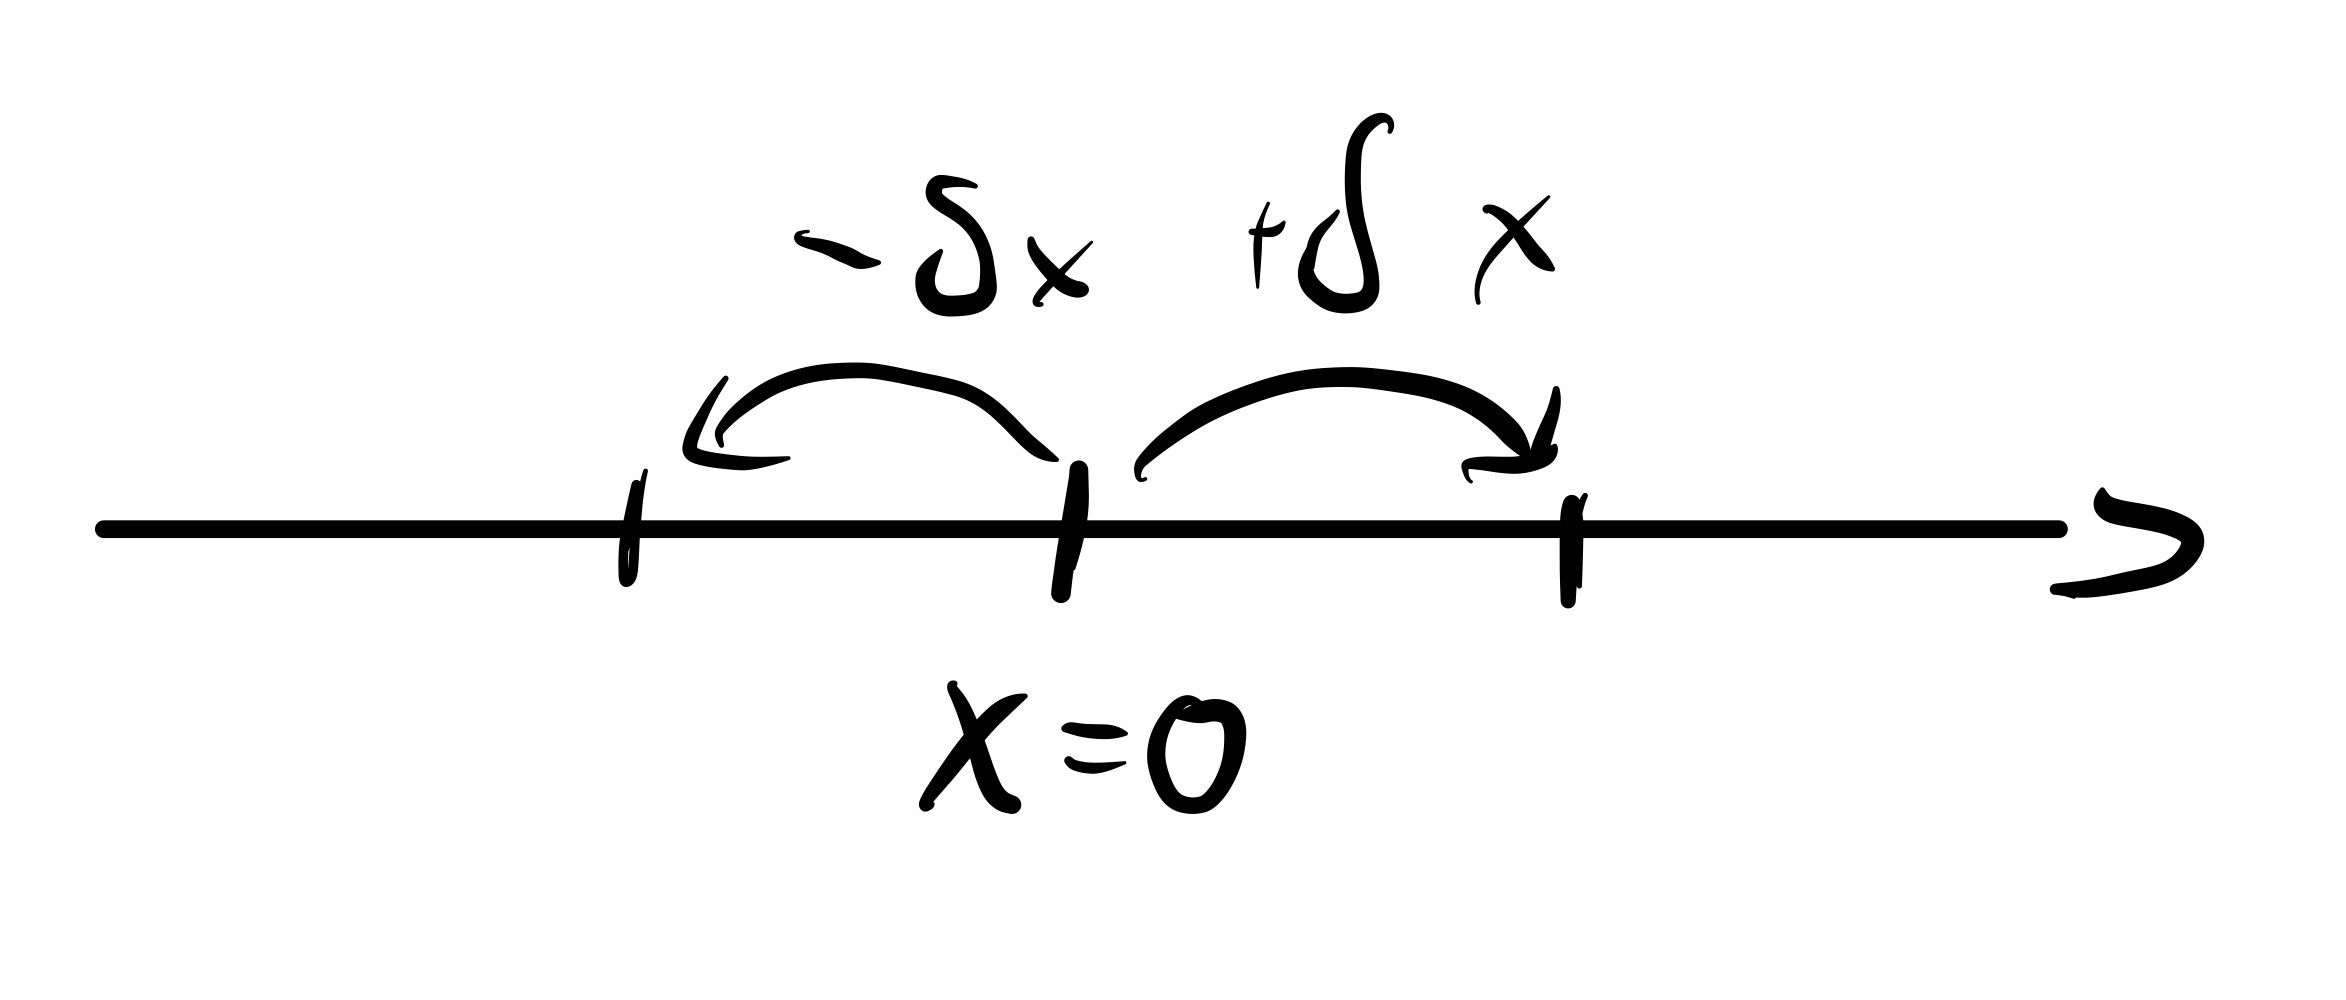
\includegraphics[width=0.8\linewidth]{Wyk_2_Rys_1.jpeg}
    \caption{Położenie cząstki}
    \label{fig:lec_2:czastka}
\end{figure}

Skoki o $\delta x$ następują co $\delta t$ i mamy:
\[ \Delta x = \begin{cases}
    \delta x \qc \frac{1}{2} \\
    - \delta x \qc \frac{1}{2}
\end{cases}\]

\begin{align*}
    x(n) = x(n-1) + \Delta x\\
    \expval{x(n)} = \expval{x(n-1)} = \expval{x(n-2)} \dots = \expval{x(0)} = 0
\end{align*}

Wynika, że:
\begin{align*}
    x(n)^2 = (x(n-1) + \Delta x)^2 = x^2(n-1) + 2x(n-1)\Delta x + (\Delta x)^2\\
    \expval{x^2(n)} = \expval{x^2(n-1)} + 2\expval{x(n-1)\Delta x} + \expval{(\Delta x)^2}
\end{align*}

Gdzie wiemy, że $2\expval{x(n-1)\Delta x} = 0$  bo kolejne skoki są niezależne, a $\expval{(\Delta x)^2} = (\delta x)^2$

Czyli:
\begin{align*}
    \expval{x^2(n)} = \expval{x^2(n-1) + (\delta x)^2}\\
    \expval{x^2(n)} = n (\delta x)^2 + \expval{x^2(0)}
\end{align*}
Ale $\expval{x^2(0)} = 0$, więc widzimy, że:
\[
    \expval{x(n)} = 0 \qc \expval{x^2(n)} = n (\delta x)^2
\]
Teraz oznaczmy sobie $n = \frac{T}{\delta t}$, a $\frac{(\delta x)^2}{2 \delta t} = D$ - stała dyfuzji. Wtedy dostajemy ruch dyfuzyjny (\ind{Ruch Browna}).
\[
    \expval{x^2(n)} = 2 T \frac{(\delta x)^2}{2 \delta t}
\]
Dokładna definicja ruchu Browna to:
\[
    \text{ruch Browna} = 
    \begin{cases}
    \expval{x^2(n)} = 2 D T \\
    \expval{x(n)} = 0
    \end{cases}\qq{gdzie}
    x = vt\qc t=\frac{L}{v}\qc T=\frac{L^2}{2D}
\] gdzie $L$ - odległość.

Przykładowe wartości:\\
\emph{Bakteria} - $L \sim 10^{-4}$ wtedy $D \sim 10^{-5} \frac{cm^2}{s}$ a czas dyfuzji $t = \frac{L^2}{2 D} = 5 \cdot 10^{-4} \sim (0.5)\,$ms
ale np z jednogo końca auli na drugi szło by to miesiąc.\\
\emph{Takeaway} - Zapachy nie transportują się dyfuzyjnie!

\section{Równanie Master}

\begin{figure}[!ht]
    \centering
    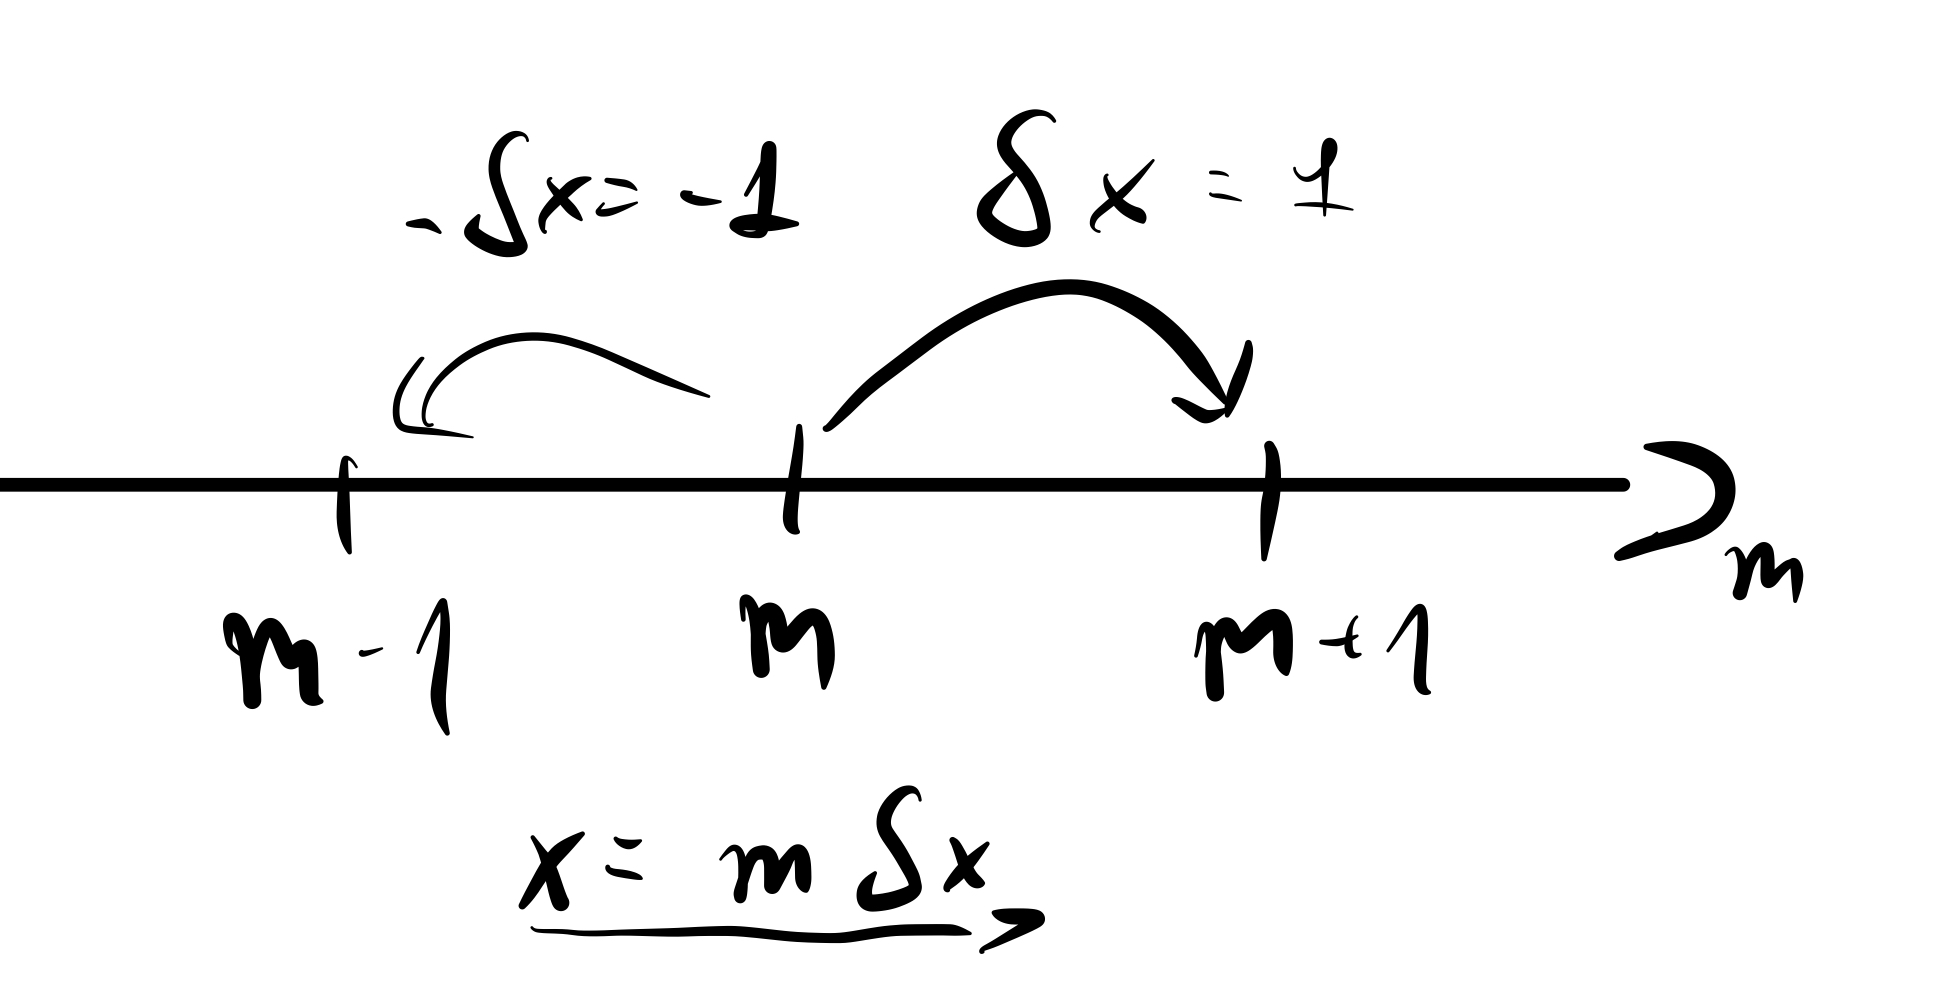
\includegraphics[width=0.8\linewidth]{Wyk_2_Rys_2.jpeg}
\end{figure}

$x = m \delta x \to$, $t \pm 1 = t \pm \delta t$

\begin{align*}
    P(m, t+1) &= \frac12 P(m+1, t) + \frac12 P(m-1, t )\\
    P(m, t+1) - P(m, t) &= \frac12(P(x + \delta x, t) - 2P(x, t) + P(x - \delta x, t))\\ 
    \qq{co jest drugą pochodną w punkcie}x:&\\
    P(m, t+1) - P(m, t) &= \frac12\delta x\qty(\frac{P(x + \delta x, t) - P(x, t)}{\delta x} - \frac{P(x, t) - P(x - \delta x, t)}{\delta x})\\
    P(m, t+1) - P(m, t) &= \frac12(\delta x)^2\qty(P'\qty(x + \frac{\delta x}{2}, t) - P'\qty(x - \frac{\delta x}{2}, t))\\
    \qq{co na mocy \textit{central limit theorem}}& \text{tłumaczy się na:}\\
    \pdv{P}{t} &= \frac{P(x, t+\delta t) - P(x, t)}{\delta t} = \frac{(\delta x)^2}{\delta t}\pdv[2]{P}{x}\\
    \qq{po przejściu do granic:} &\delta t \to 0\qc \delta x \to 0\qc \frac{\delta x^2}{\delta t} = \qq{const.}\\
\end{align*}
Dostajemy równanie dyfuzji:
\begin{equation}
    \pdv{P}{t} = D \pdv[2]{P}{x}
    \label{eq:lec_2:dyfuzja}
\end{equation}
Co dla
\[
    P(x, t=0) = \delta(x)
\]
Daje nam rozkład prawdopodobieństwa występowania punktu w jakimś $x$ przy dyfuzji wygląda:
\begin{equation}
    P(x) = \frac{1}{\sqrt{4 \pi D t}} e^{-\frac{x^2}{4 D t}}
    \label{eq:lec_2:rozklad_gauss}
\end{equation}
Czyli rozkład Gaussa, widoczny na Rysunku \ref{fig:lec_2:mol_pow}.

\section{Demonstracje}
\begin{figure}[!ht]
    \centering
    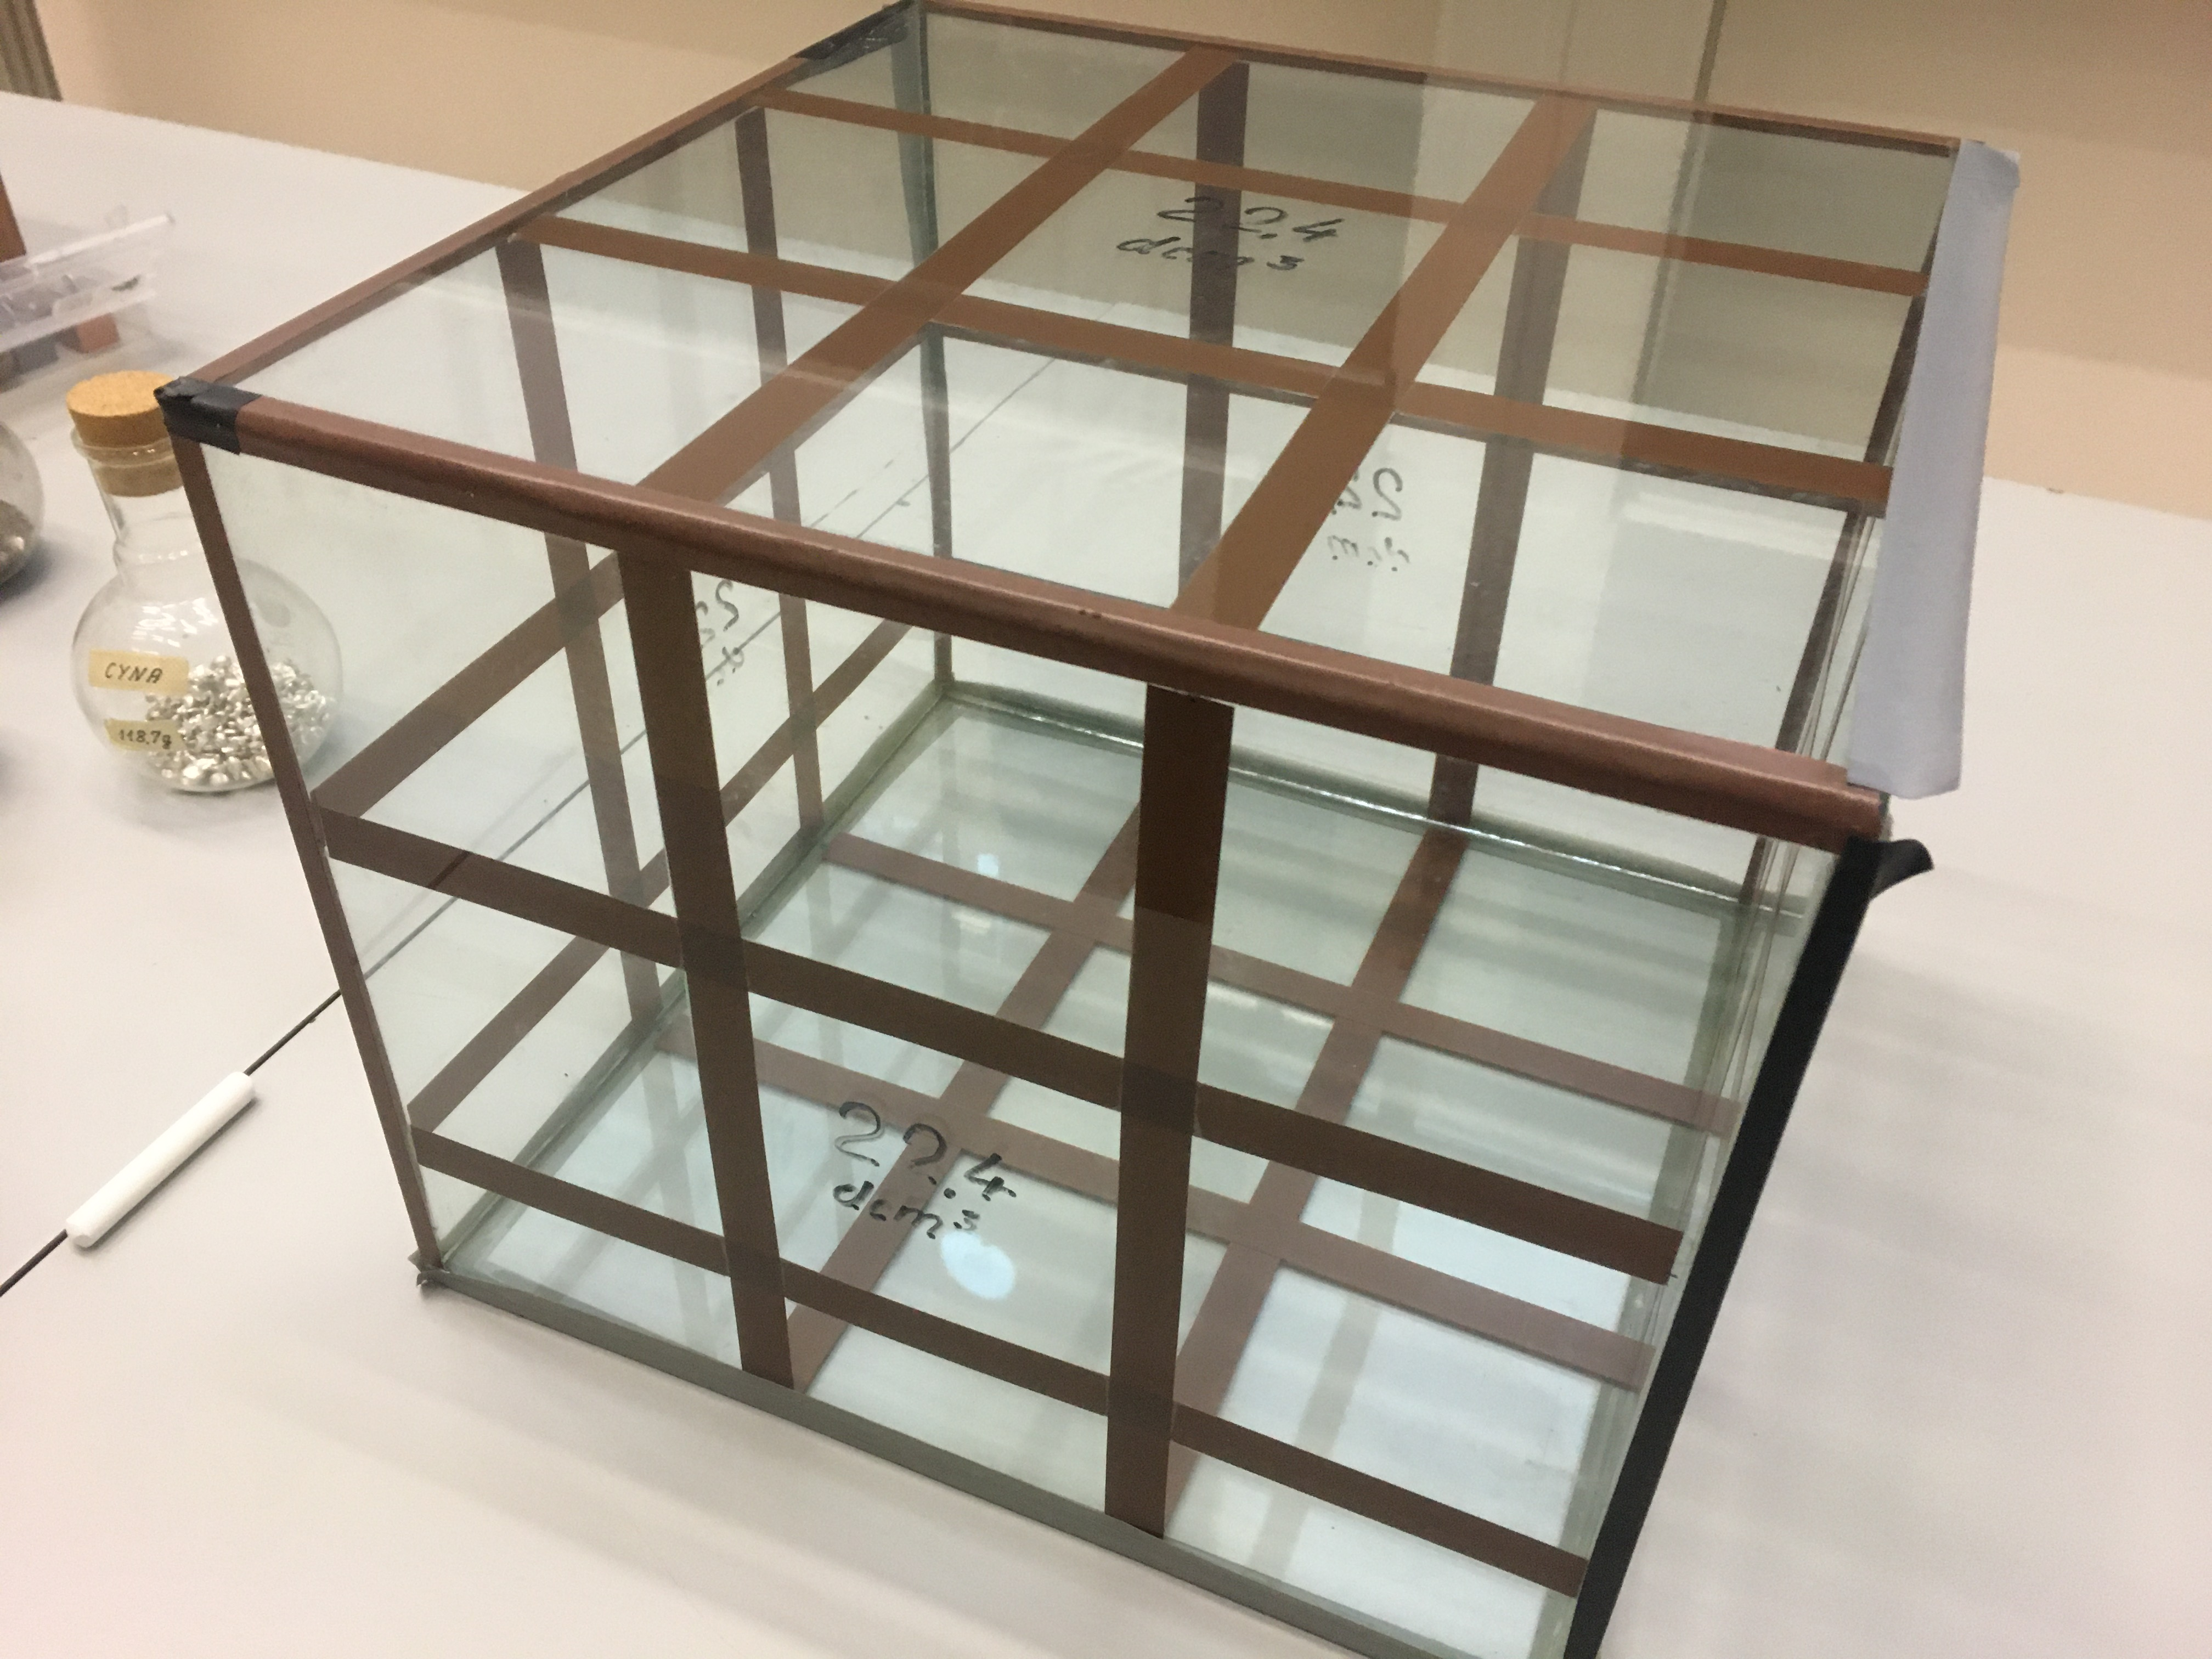
\includegraphics[width=0.5\linewidth]{Wyk_2_Rys_3.JPG}
    \caption{Jeden mol powietrza}
    \label{fig:lec_2:mol_pow}
\end{figure}

\begin{figure}[!ht]
    \centering
    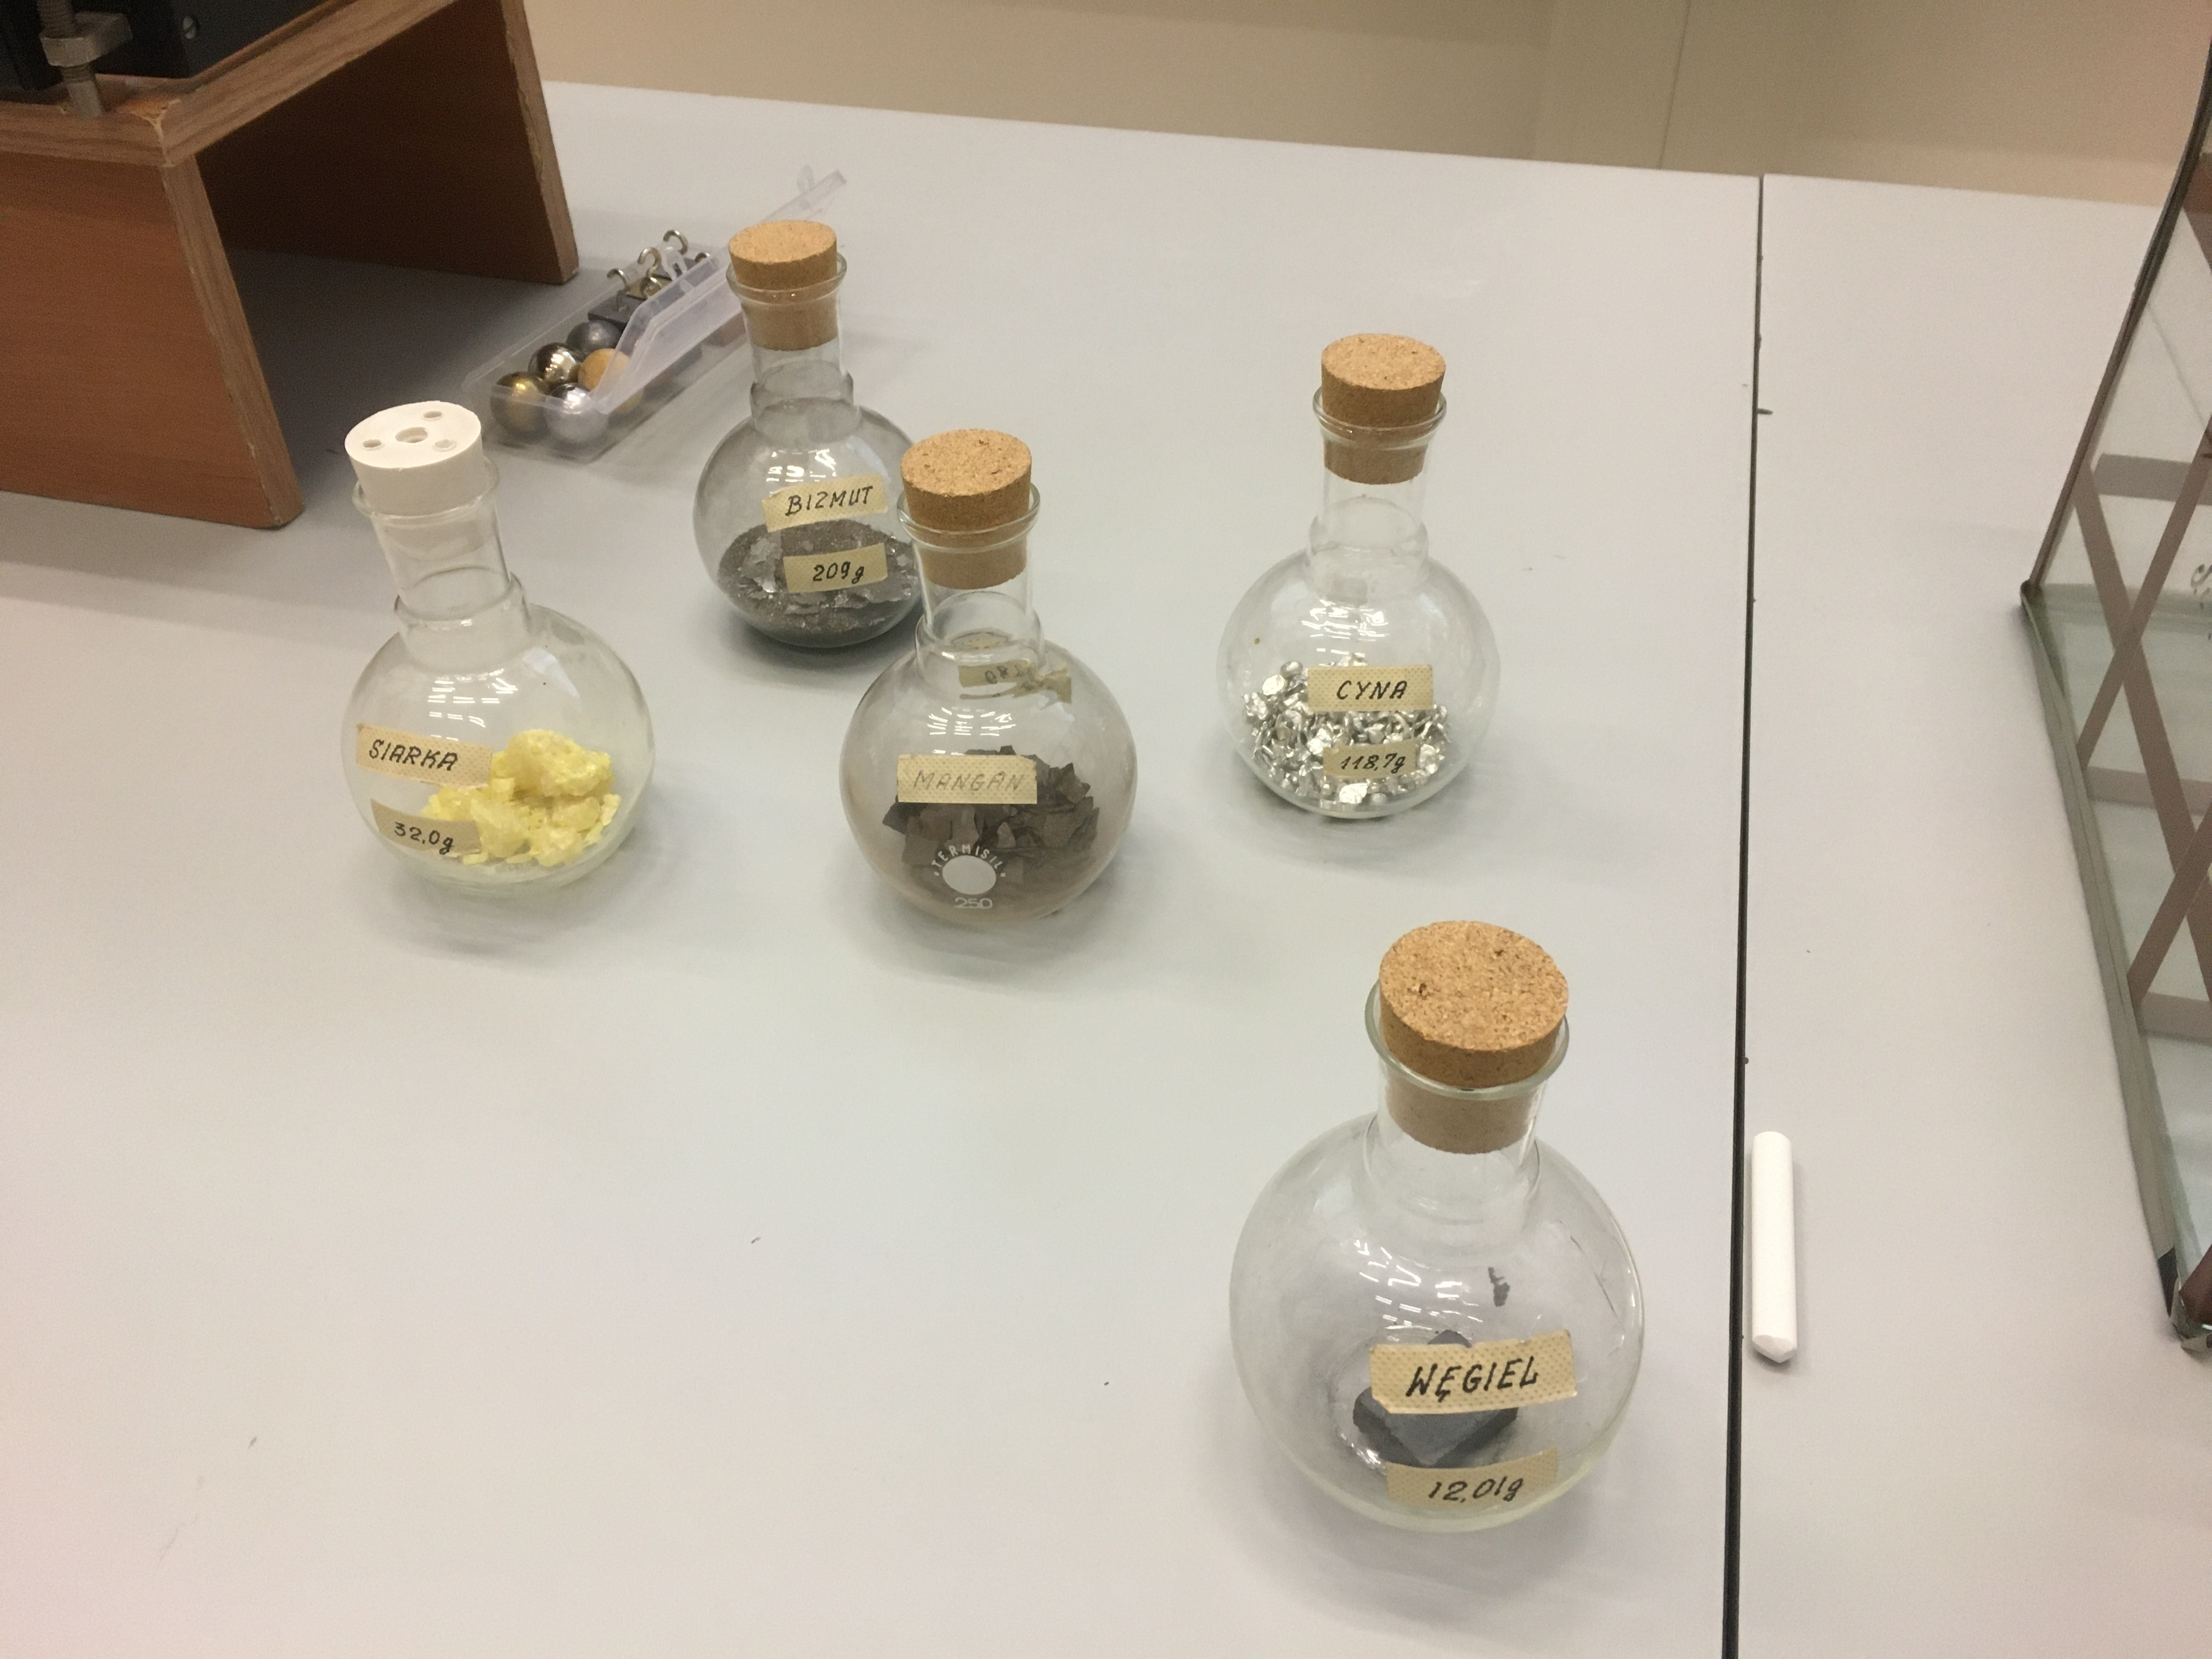
\includegraphics[width=0.8\linewidth]{Wyk_2_Rys_4.JPG}
    \caption{Jeden mol innych rzeczy}s
    \label{fig:lec_2:mole_demo}
\end{figure}

\begin{figure}[!ht]
    \centering
    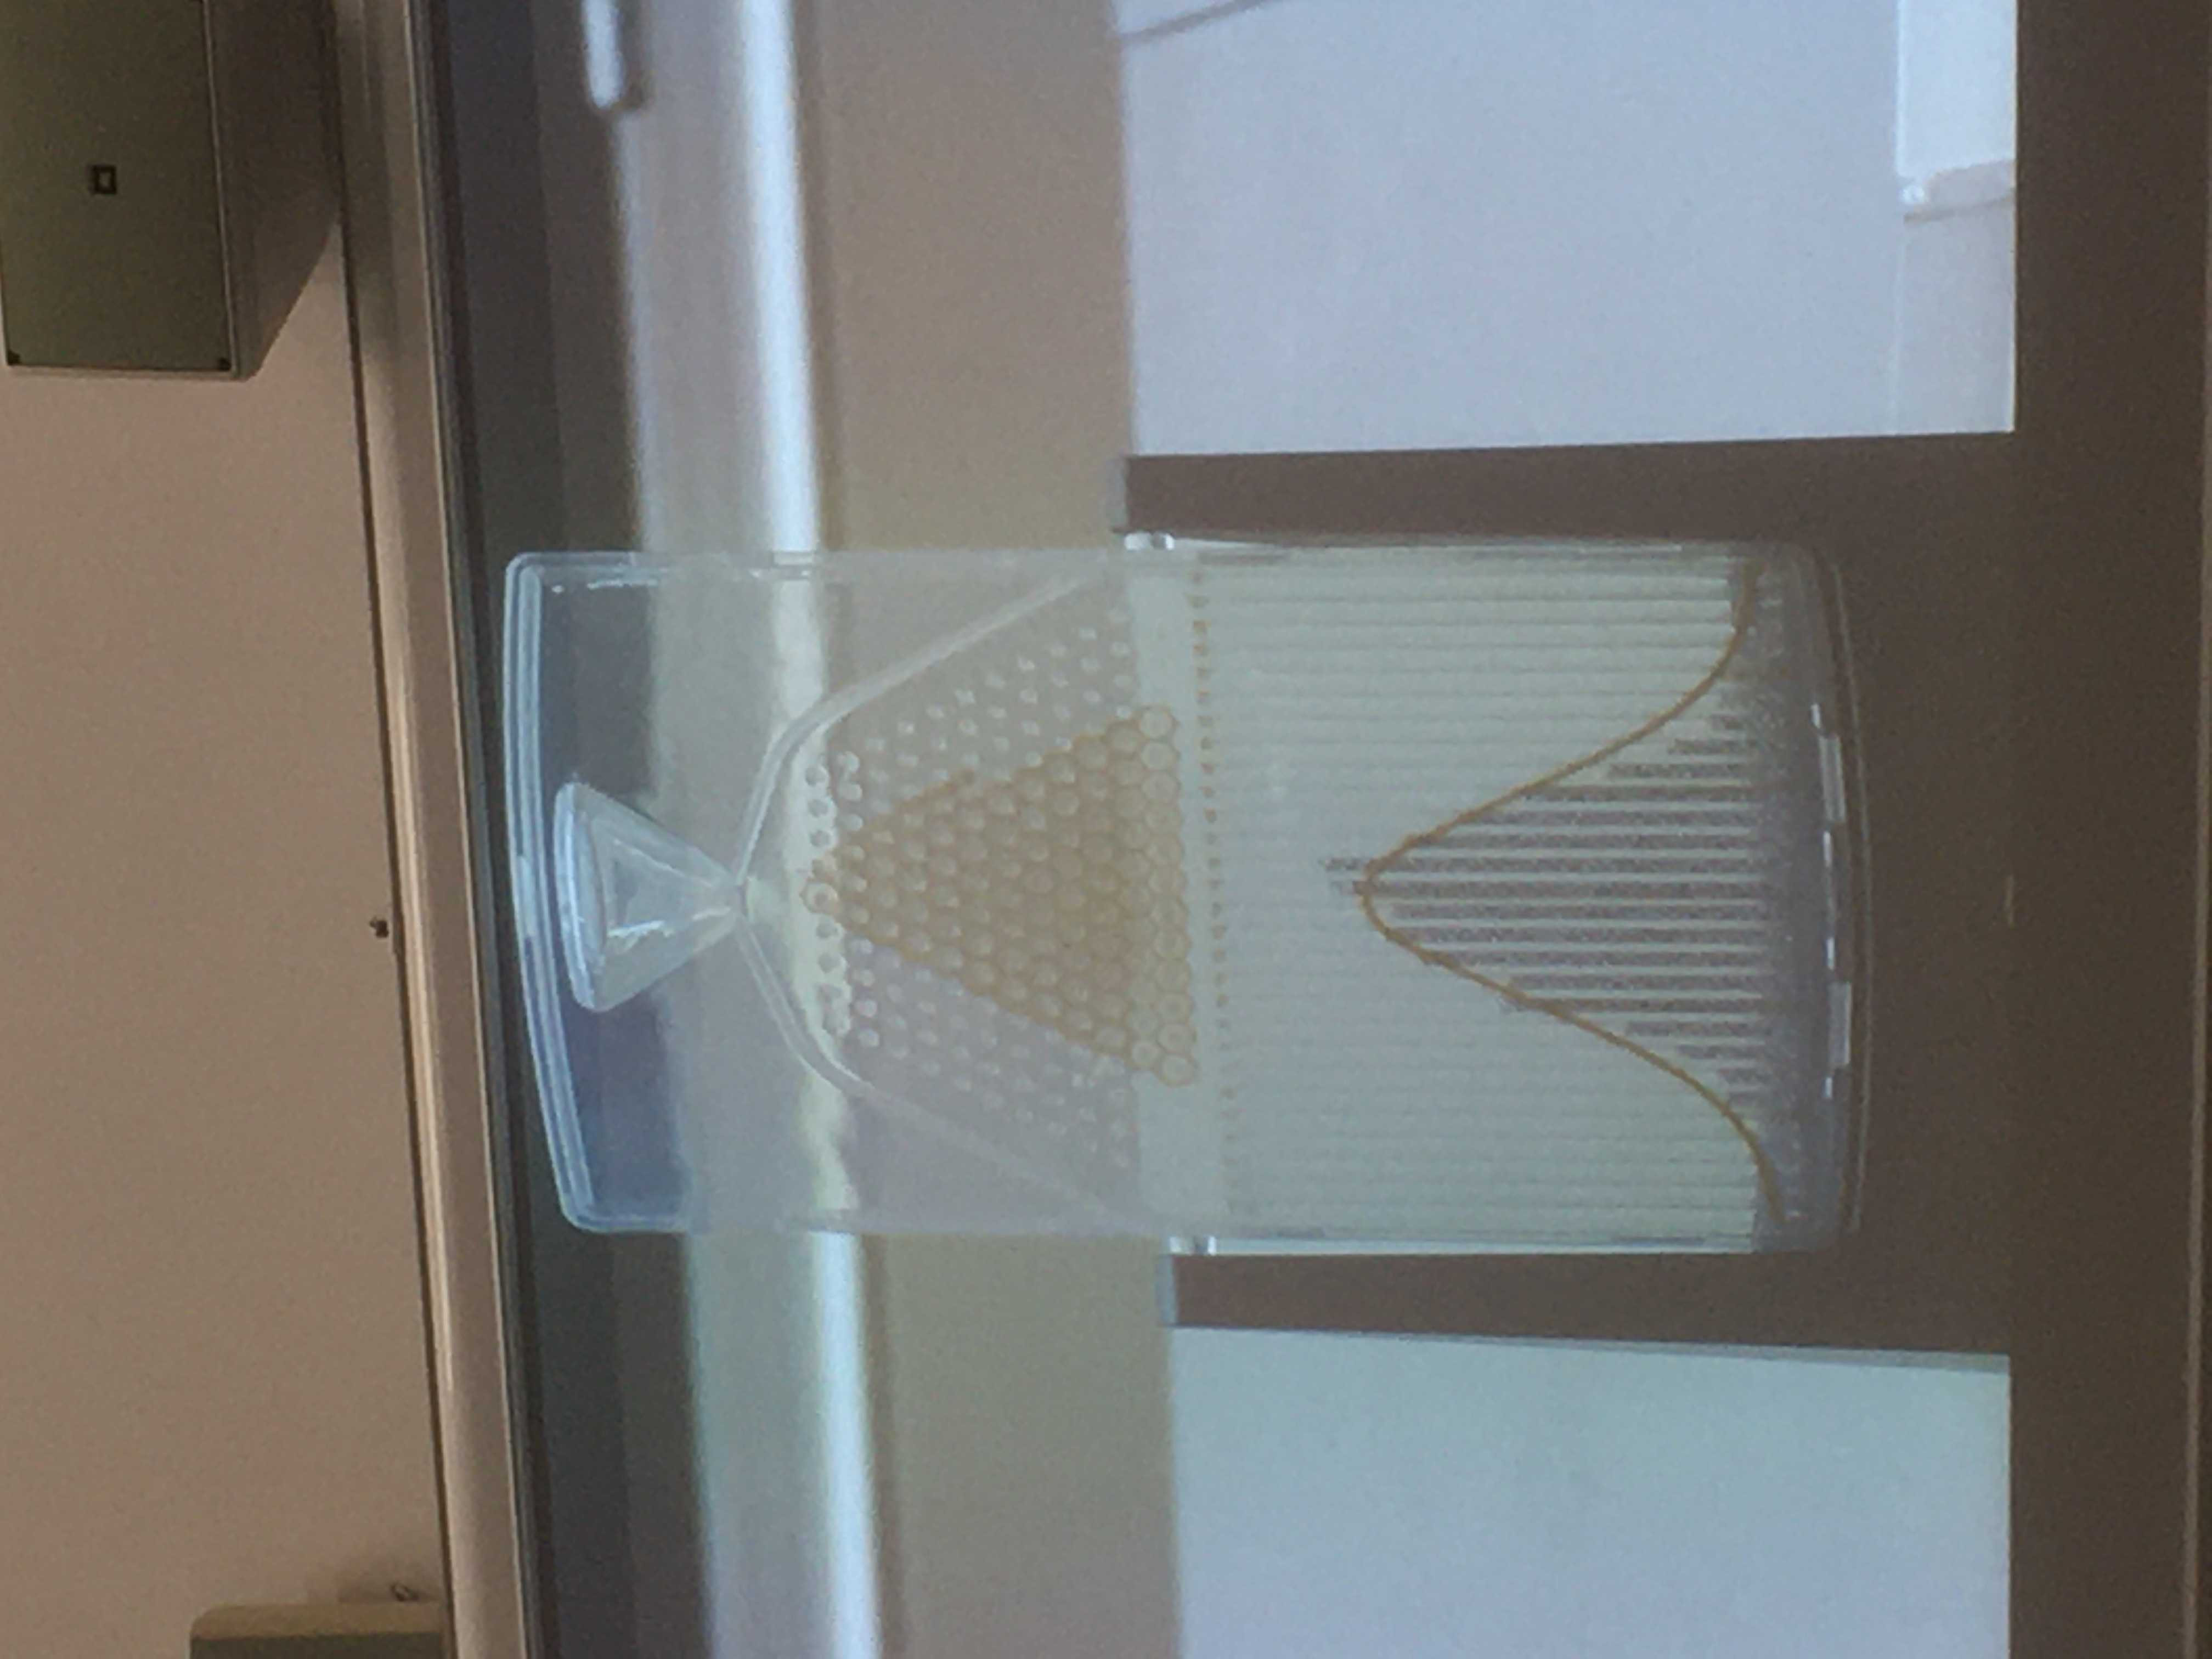
\includegraphics[width=0.8\linewidth, angle=270]{Wyk_2_Rys_5.JPG}
    \caption{Przykładowy \ind{Rozkład Gaussa} uzyskany ze spadających kulek}
    \label{fig:lec_2:gauss}
\end{figure}

Teaser na przyszłość, dyfuzja z dodatkowym członem od pola siły.
\begin{equation}
    \pdv{P}{t} = D \pdv[2]{P}{x} - \pdv{F}{\gamma}P
    \label{eq:lec_2:dyfuzja_pelna}
\end{equation}

\FloatBarrier

\section{Wracamy do Modelu Erhnferstów}

\begin{align}
    P(n, t+1) = \frac{n+1}{N} P(n+1, t)+ (1 - \frac{n-1}{N}) P(n-1, t) \label{eq:lec_2:Psy_1}\\
    P(0, t+1) = \frac1N P(1, t)\label{eq:lec_2:Psy_2}\\
    P(N, t+1) = (1 - \frac{N - 1}{N}) P( N-1, t)\label{eq:lec_2:Psy_3}
\end{align}
Szukamy rozwiązania niezależnego od czasu - $p^{eq}(n)$. Z równania \ref{eq:lec_2:Psy_2} wynika:
\begin{align*}
    p^{eq}(0) &= a\qc p^{eq}(1) = N\qc p^{eq}(n) = \mqty(N \\ n)a\\
    &\qq{\color{purple} Udowodnijmy przez indukcję:}\\
    &\begin{cases}
        p^{eq}(n-1) = a \mqty(N \\ n-1)\\
        p^{eq}(n) = a \mqty(N \\n)
    \end{cases}\\
    &\qq{\color{purple} Teraz biorąc równanie \ref{eq:lec_2:Psy_1} wyżej:}\\
    p^{eq}(n+1) \frac{n+1}{N} &= a \qty[\mqty(N \\ n) \mqty(N \\ n-1) \frac{N - n +1}{N}]\\ \\ \hline \hline
    &\qq{\color{purple}Pamiętając o tożsamości:}\\
    \mqty(N \\n) &= \mqty(N-1 \\ n) + \mqty(N-1 \\ n-1)\qq{dostajemy:}\\ \hline \hline \\
    p^{eq}(n+1) &= a \frac{N}{n +1}\qty[\qty{\mqty(N-1\\n) + \mqty(N-1 \\ n-1)} - \qty{\mqty(N-1 \\ n-1) + \mqty(N -1 \\ n-2)} \cdot \frac{N - n + 1}{N}]\\
    p^{eq}(n+1) &= a \frac{N}{n +1} \qty[\frac{(N-1)! N }{n! (N-1-n)! (n+1)} + \frac{(N-1)!}{(n-2)!(N-n)!(n+1)} - \frac{(N-1!)}{(n-2)!(N-n)! (n+1)}]\\
    p^{eq}(n+1) &= a\mqty(N \\ n+1)
\end{align*}

\end{lecture}

\tableofcontents

\listoffigures

\printindex

\end{document}